\appendix
\chapter{Appendix}

\section{Dependencies}
\label{sec:dependencies}

A complete list of python packages used for the implementation and experiments:

\begin{itemize}
    \item Babel version 2.9.1
    \item kmeans\_pytorch version 0.3
    \item matplotlib version 3.3.4
    \item numpy version 1.20.2
    \item pandas version 1.2.4
    \item Pillow version 8.2.0
    \item rsa version 4.7.2
    \item torch version 1.8.1
    \item torchvision version 0.9.1
\end{itemize}

\section{Additional figures}
\label{sec:appendix:additional-figures}
\subsection{Experiments for fine-tuning} \label{sec:appendix:finetuning-plots}
%%%%%%%%%%%%%%%%%%%%%%%%%%%%%%%%%%%%%%%%%%% MNIST models
\begin{figure}
     \centering
     \begin{subfigure}[b]{0.49\textwidth}
         \centering
         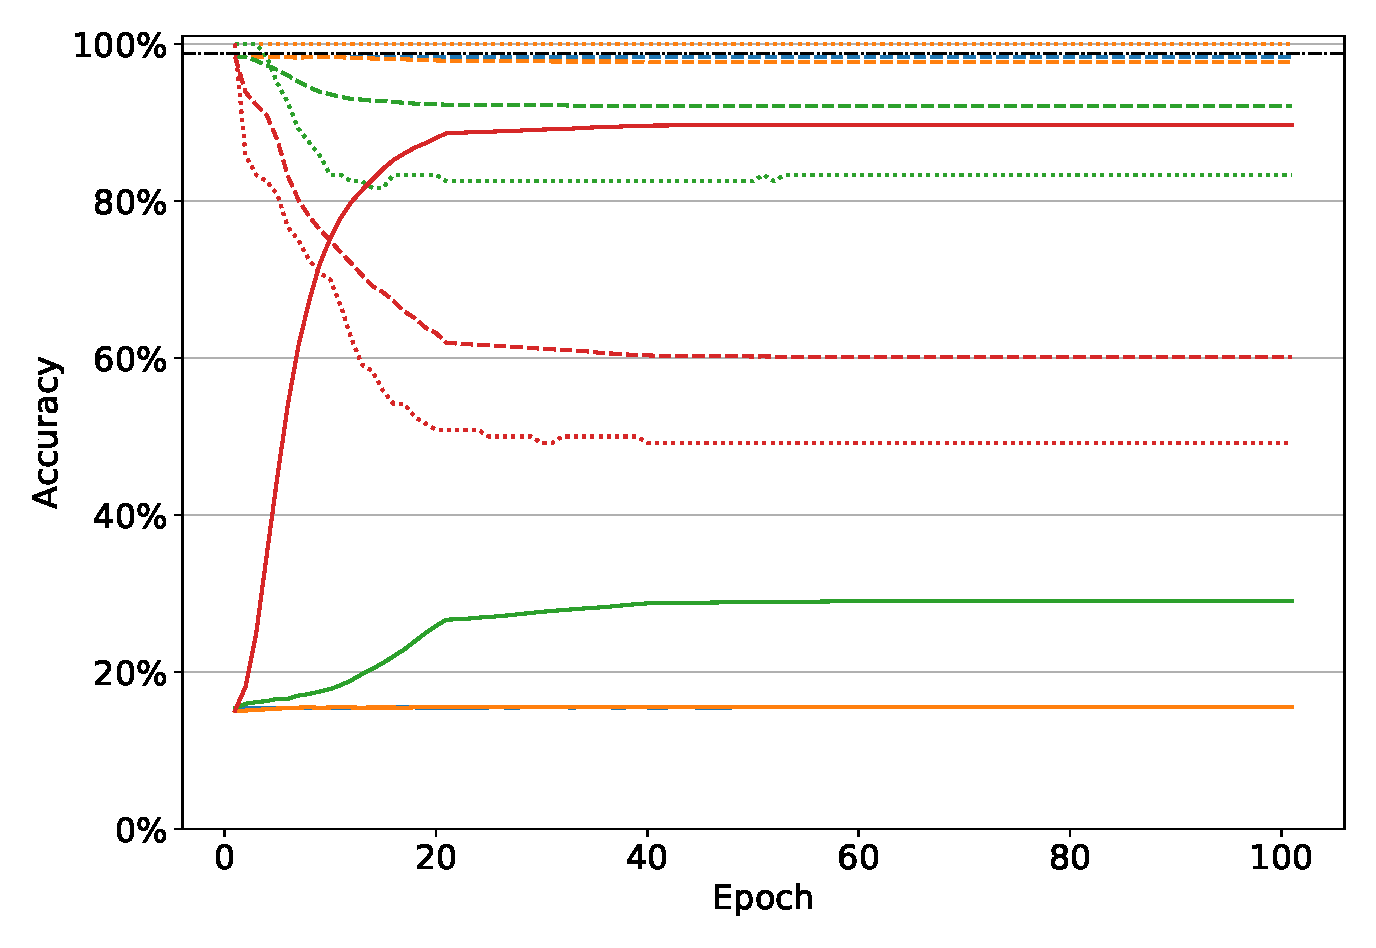
\includegraphics[width=\textwidth]{images/finetuning/finetuning_protecting_content_smalllr_thesis_lenet1.eps}
         \caption{LeNet-1}
         \label{fig:finetuning_lenet1_smalllr}
     \end{subfigure}
     \hfill
     \begin{subfigure}[b]{0.49\textwidth}
         \centering
         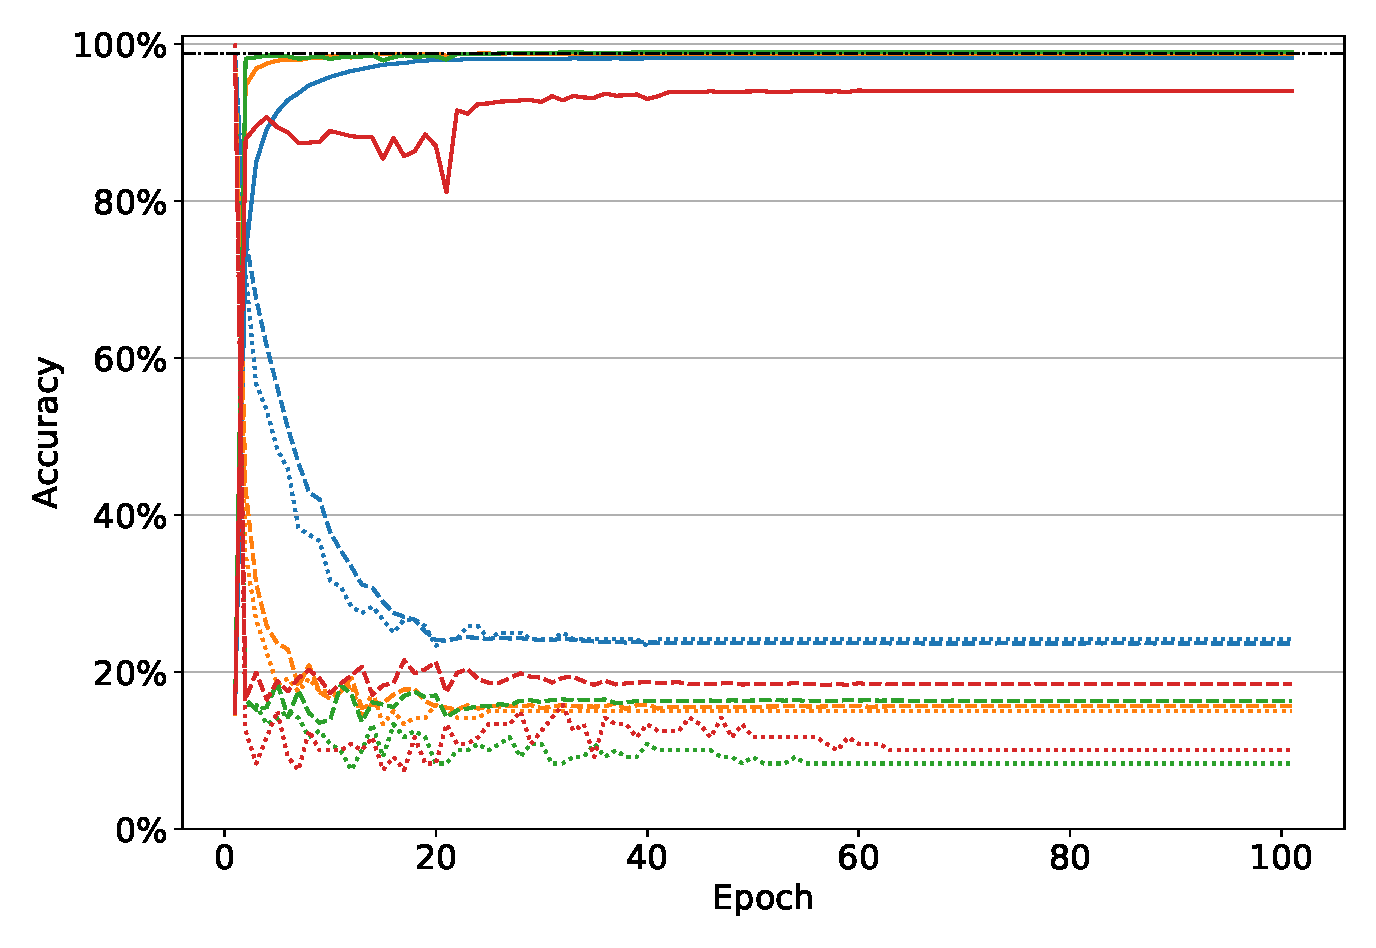
\includegraphics[width=\textwidth]{images/finetuning/finetuning_protecting_content_largelr_thesis_lenet1.eps}
         \caption{LeNet-1}
         \label{fig:finetuning_lenet1_largelr}
     \end{subfigure}
     \begin{subfigure}[b]{0.49\textwidth}
         \centering
         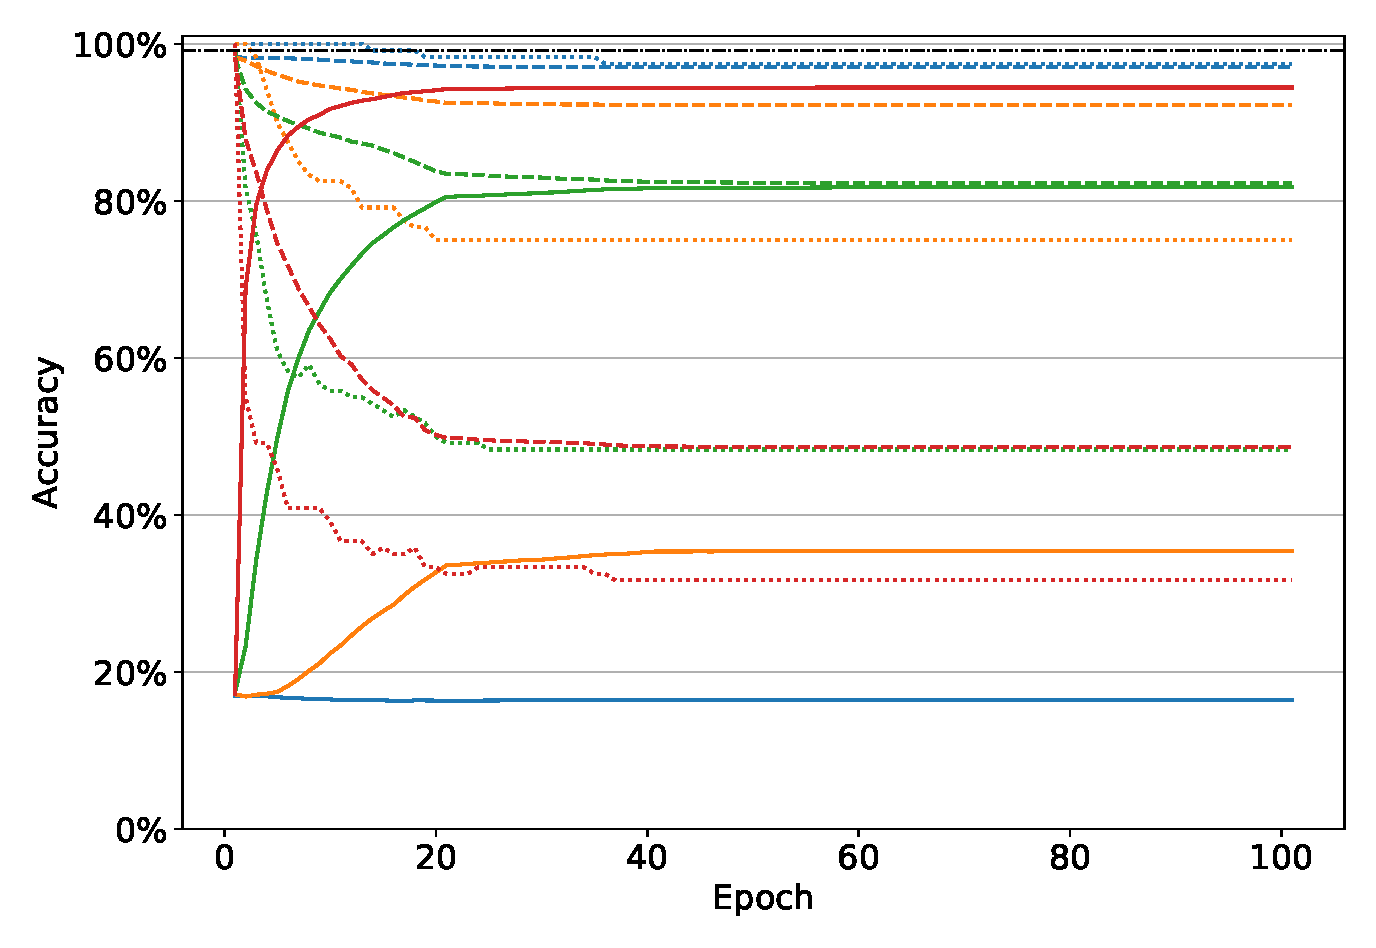
\includegraphics[width=\textwidth]{images/finetuning/finetuning_protecting_content_smalllr_thesis_lenet3.eps}
         \caption{LeNet-3}
         \label{fig:finetuning_lenet3_smalllr}
     \end{subfigure}
     \hfill
     \begin{subfigure}[b]{0.49\textwidth}
         \centering
         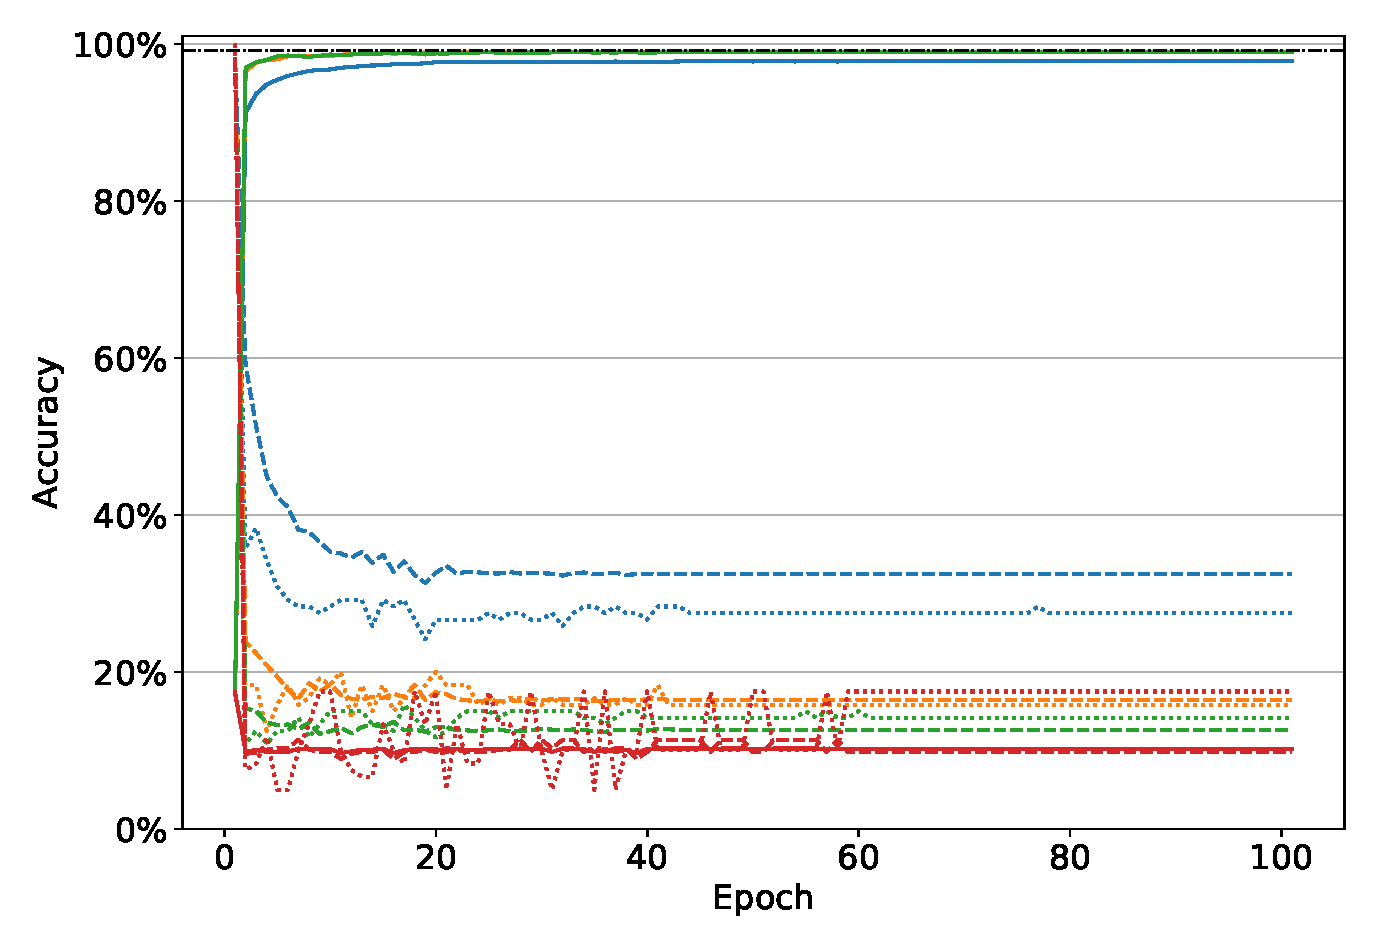
\includegraphics[width=\textwidth]{images/finetuning/finetuning_protecting_content_largelr_thesis_lenet3.eps}
         \caption{LeNet-3}
         \label{fig:finetuning_lenet3_largelr}
     \end{subfigure}
     \hfill
     \begin{subfigure}[b]{0.49\textwidth}
         \centering
         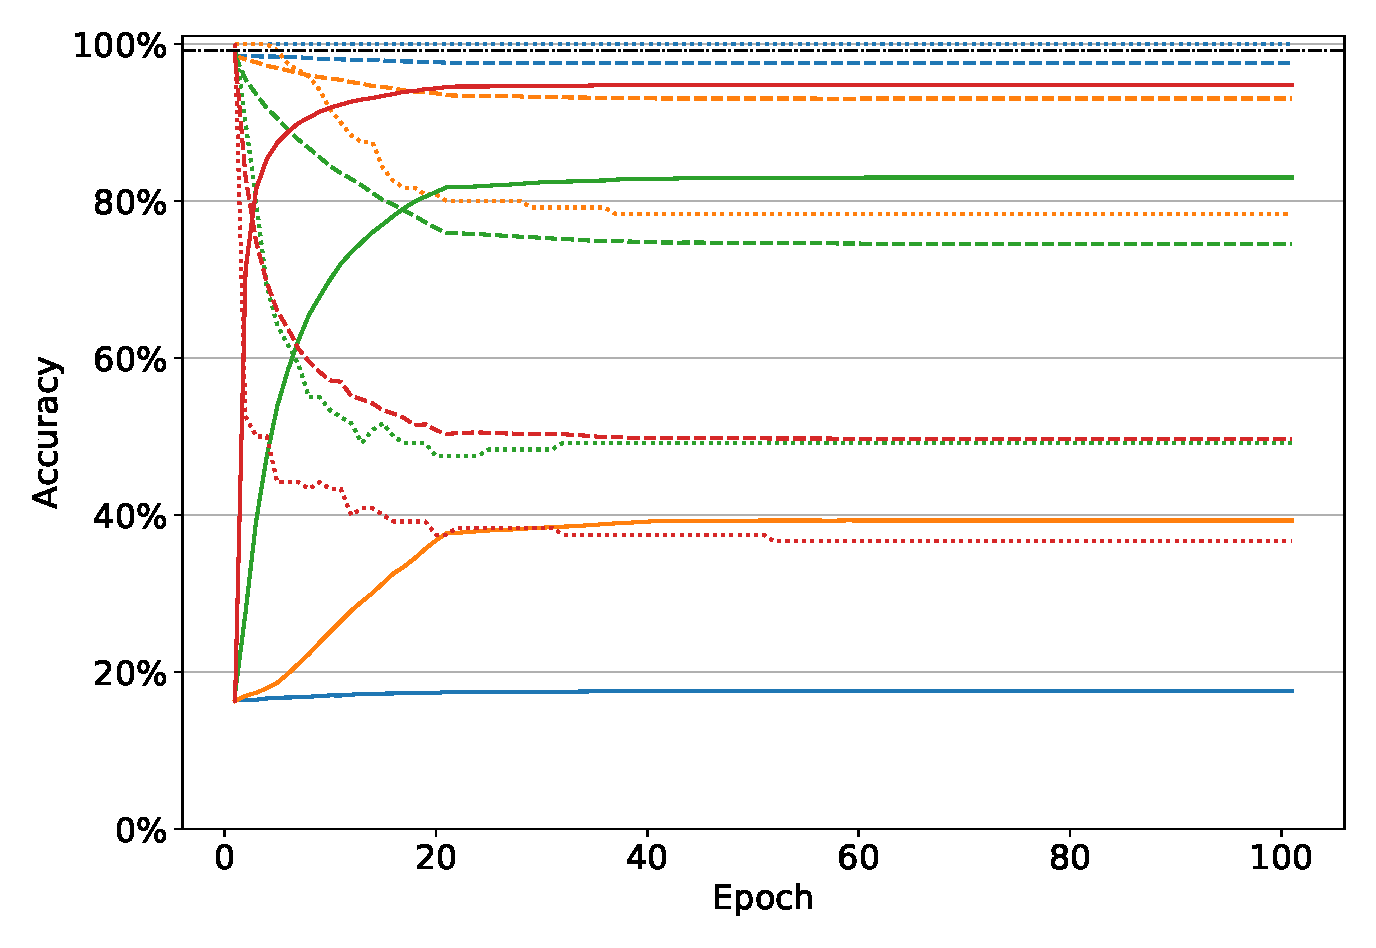
\includegraphics[width=\textwidth]{images/finetuning/finetuning_protecting_content_smalllr_thesis_lenet5.eps}
         \caption{LeNet-5}
         \label{fig:finetuning_lenet5_smalllr}
     \end{subfigure}
     \hfill
     \begin{subfigure}[b]{0.49\textwidth}
         \centering
         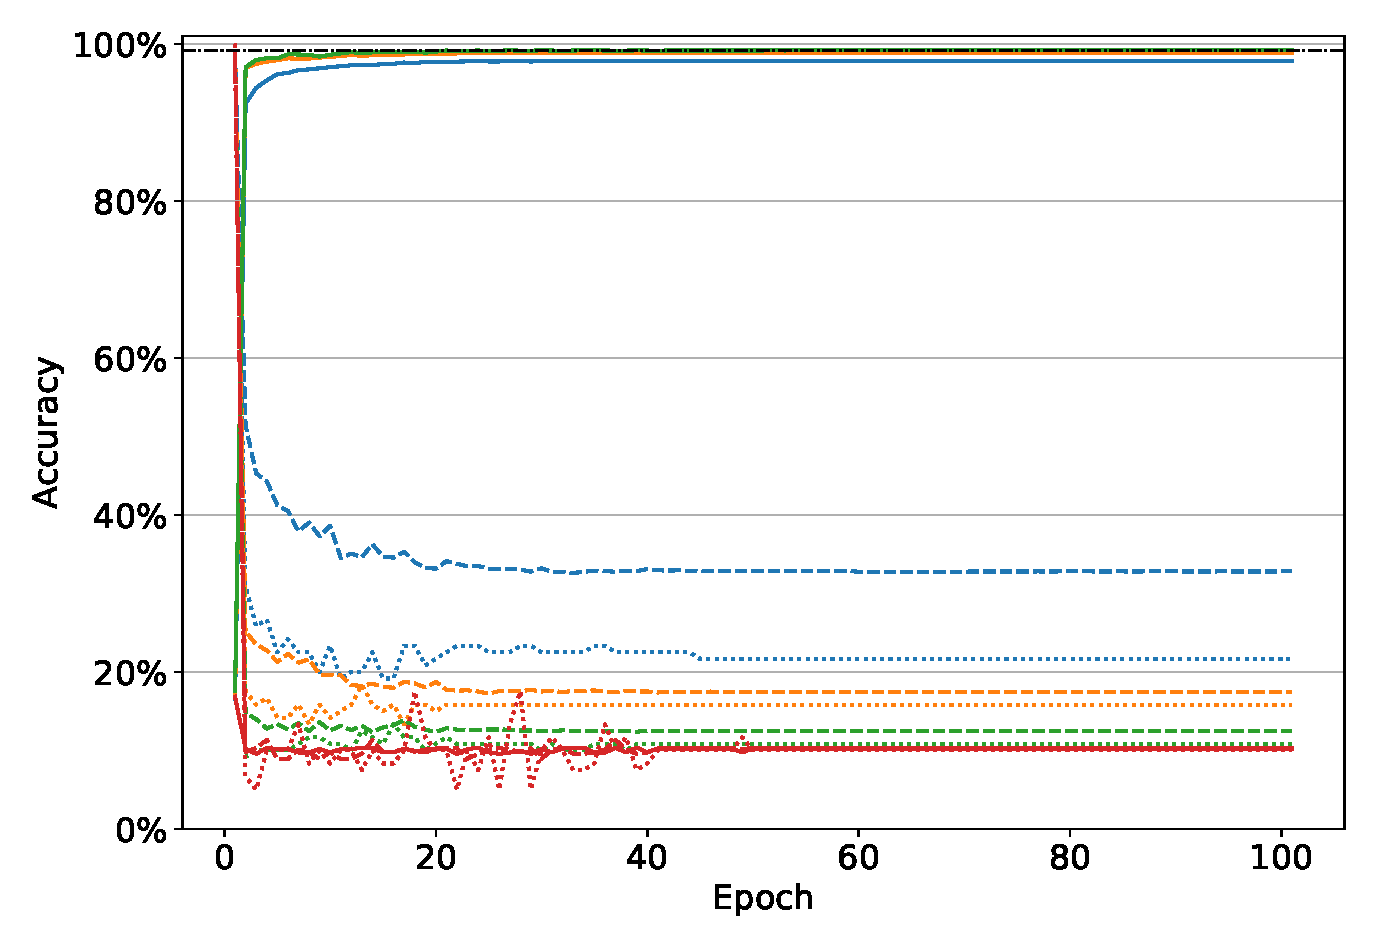
\includegraphics[width=\textwidth]{images/finetuning/finetuning_protecting_content_largelr_thesis_lenet5.eps}
         \caption{LeNet-5}
         \label{fig:finetuning_lenet5_largelr}
     \end{subfigure}
     \hfill
     
     \begin{subfigure}[b]{\textwidth}
         \centering
         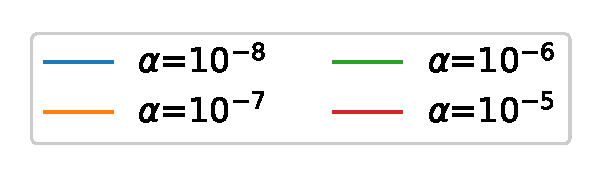
\includegraphics[height=1.1cm]{images/finetuning/legend_content_finetuning_smalllr_colors.eps}
         \quad
         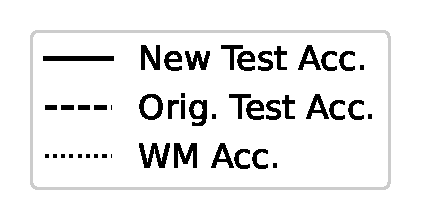
\includegraphics[height=1.3cm]{images/finetuning/legend_content_finetuning_linetypes.eps}
         \quad
         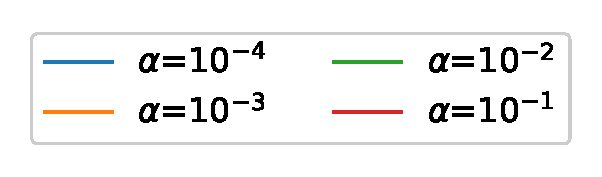
\includegraphics[height=1.1cm]{images/finetuning/legend_content_finetuning_largelr_colors.eps}
     \end{subfigure}
     
     \caption{Fine-tuning on \textbf{MNIST} models, watermarked with \textit{ProtectingIP-pattern}. The plots on the left side correspond to fine-tuning with smaller learning rates and the ones on the right side to fine-tuning with larger learning rates. The black dash-dotted line corresponds to the benchmark test accuracy of the non-watermarked model.}
     \label{fig:finetuning_mnistmodels}
\end{figure}

%%%%%%%%%%%%%%%%%%%%%%%%%%%%%%%%%%%%%%%%%%% CIFAR-10

\begin{figure}
     \centering
     \begin{subfigure}[b]{0.49\textwidth}
         \centering
         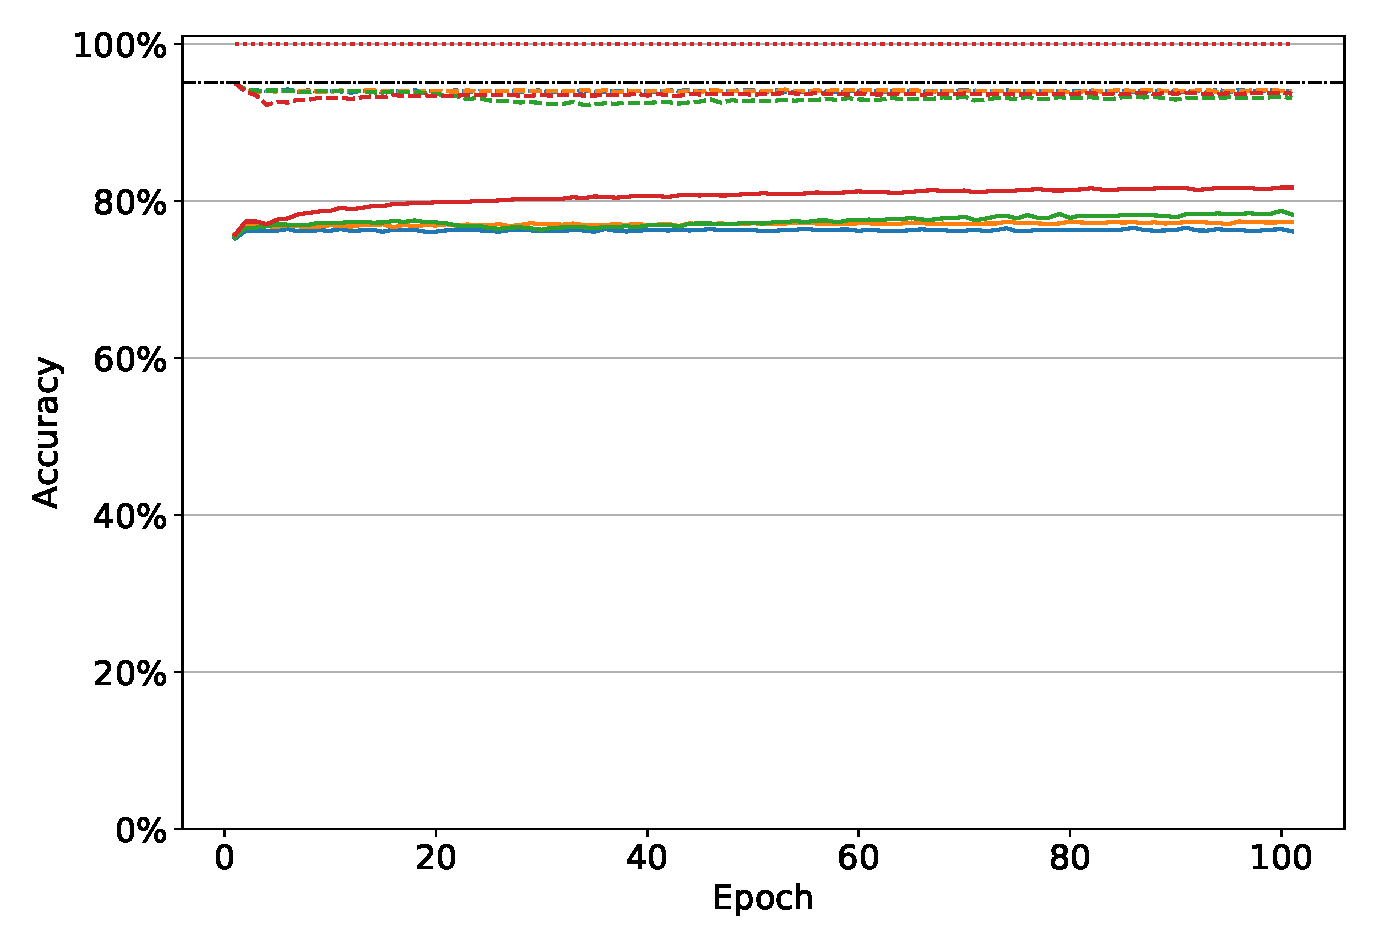
\includegraphics[width=\textwidth]{images/finetuning/finetuning_protecting_content_smalllr_thesis_resnet18.eps}
         \caption{ResNet-18}
         \label{fig:finetuning_resnet18_smalllr}
     \end{subfigure}
     \hfill
     \begin{subfigure}[b]{0.49\textwidth}
         \centering
         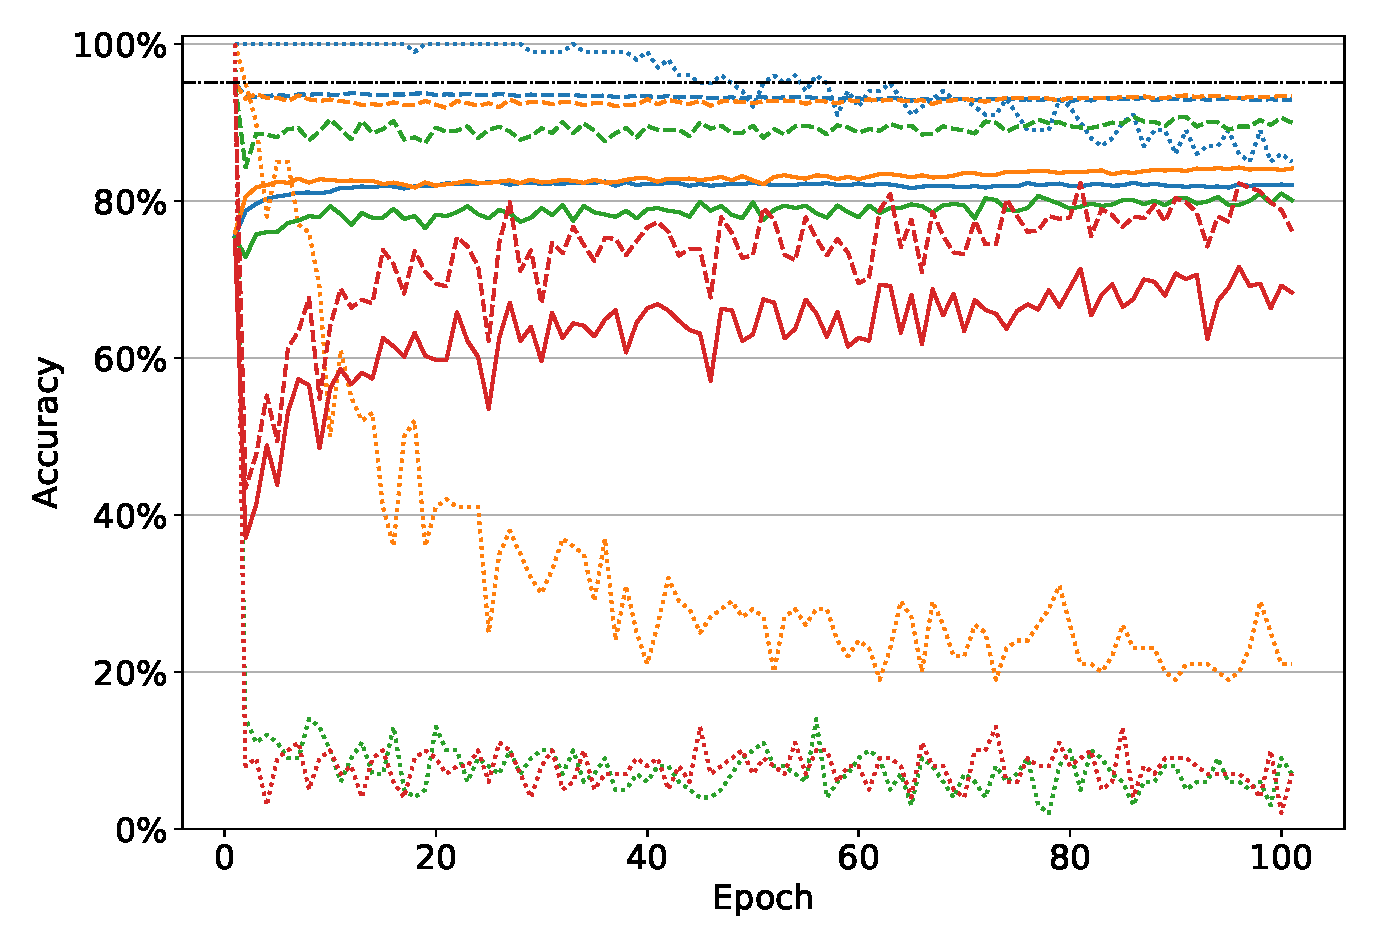
\includegraphics[width=\textwidth]{images/finetuning/finetuning_protecting_content_largelr_thesis_resnet18.eps}
         \caption{ResNet-18}
         \label{fig:finetuning_resnet18_largelr}
     \end{subfigure}
     \begin{subfigure}[b]{0.49\textwidth}
         \centering
         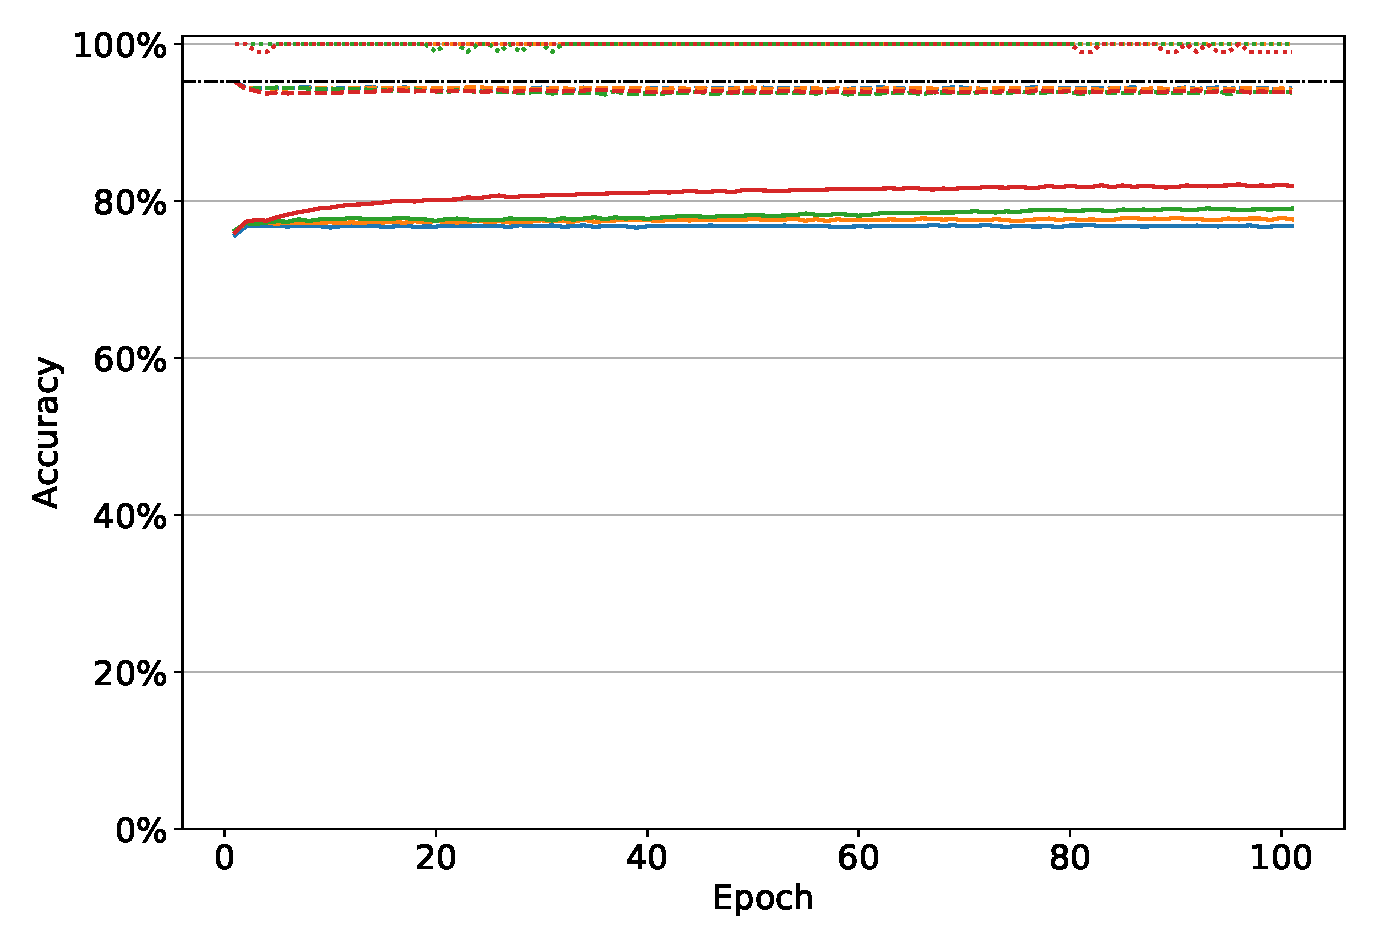
\includegraphics[width=\textwidth]{images/finetuning/finetuning_protecting_content_smalllr_thesis_resnet34.eps}
         \caption{ResNet-34}
         \label{fig:finetuning_resnet34_smalllr}
     \end{subfigure}
     \hfill
     \begin{subfigure}[b]{0.49\textwidth}
         \centering
         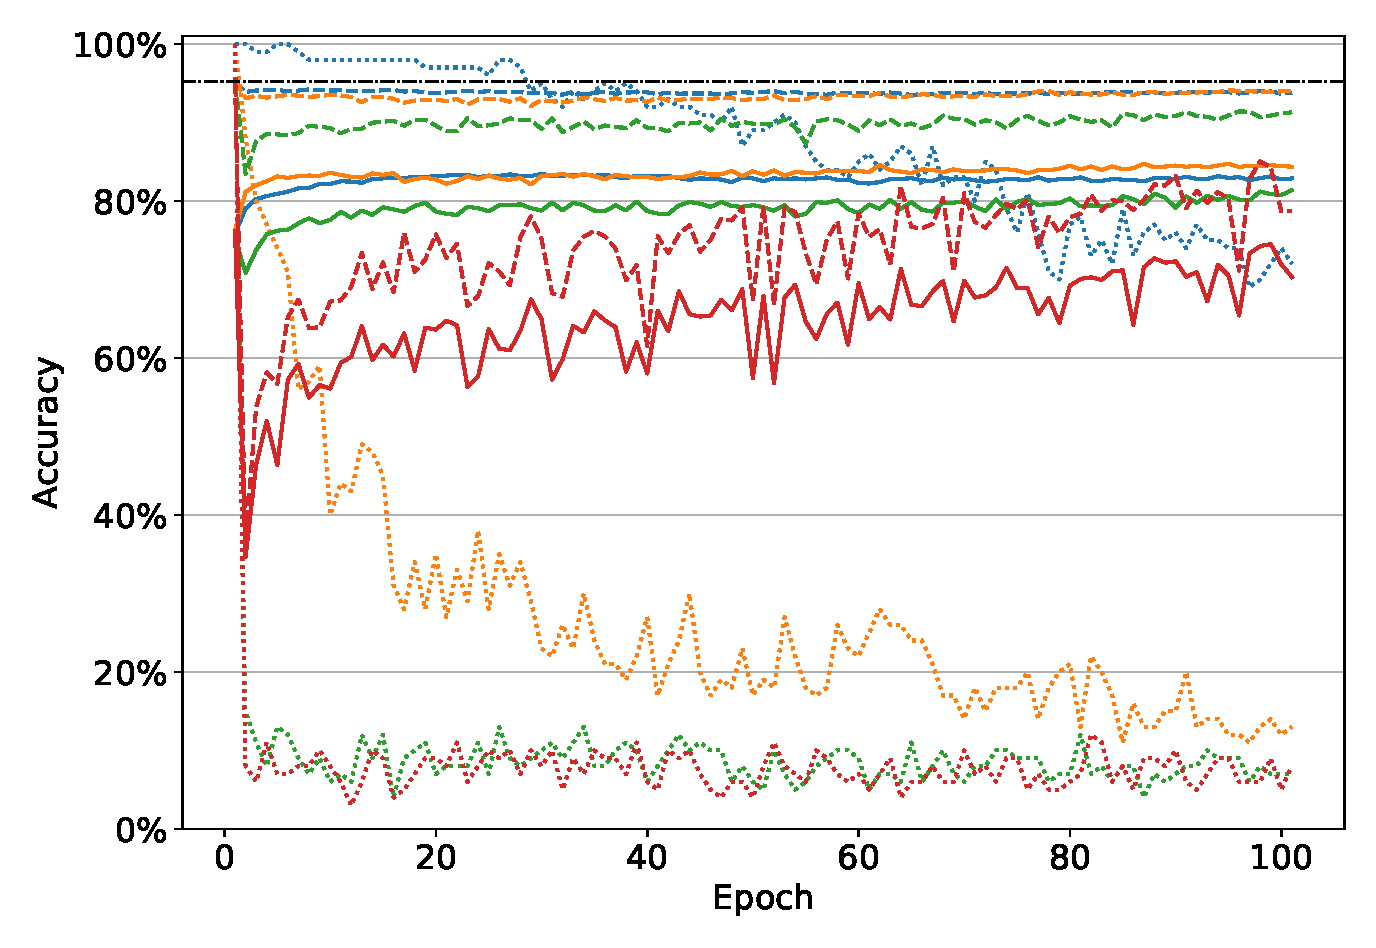
\includegraphics[width=\textwidth]{images/finetuning/finetuning_protecting_content_largelr_thesis_resnet34.eps}
         \caption{ResNet-34}
         \label{fig:finetuning_resnet34_largelr}
     \end{subfigure}
     \hfill
     \begin{subfigure}[b]{0.49\textwidth}
         \centering
         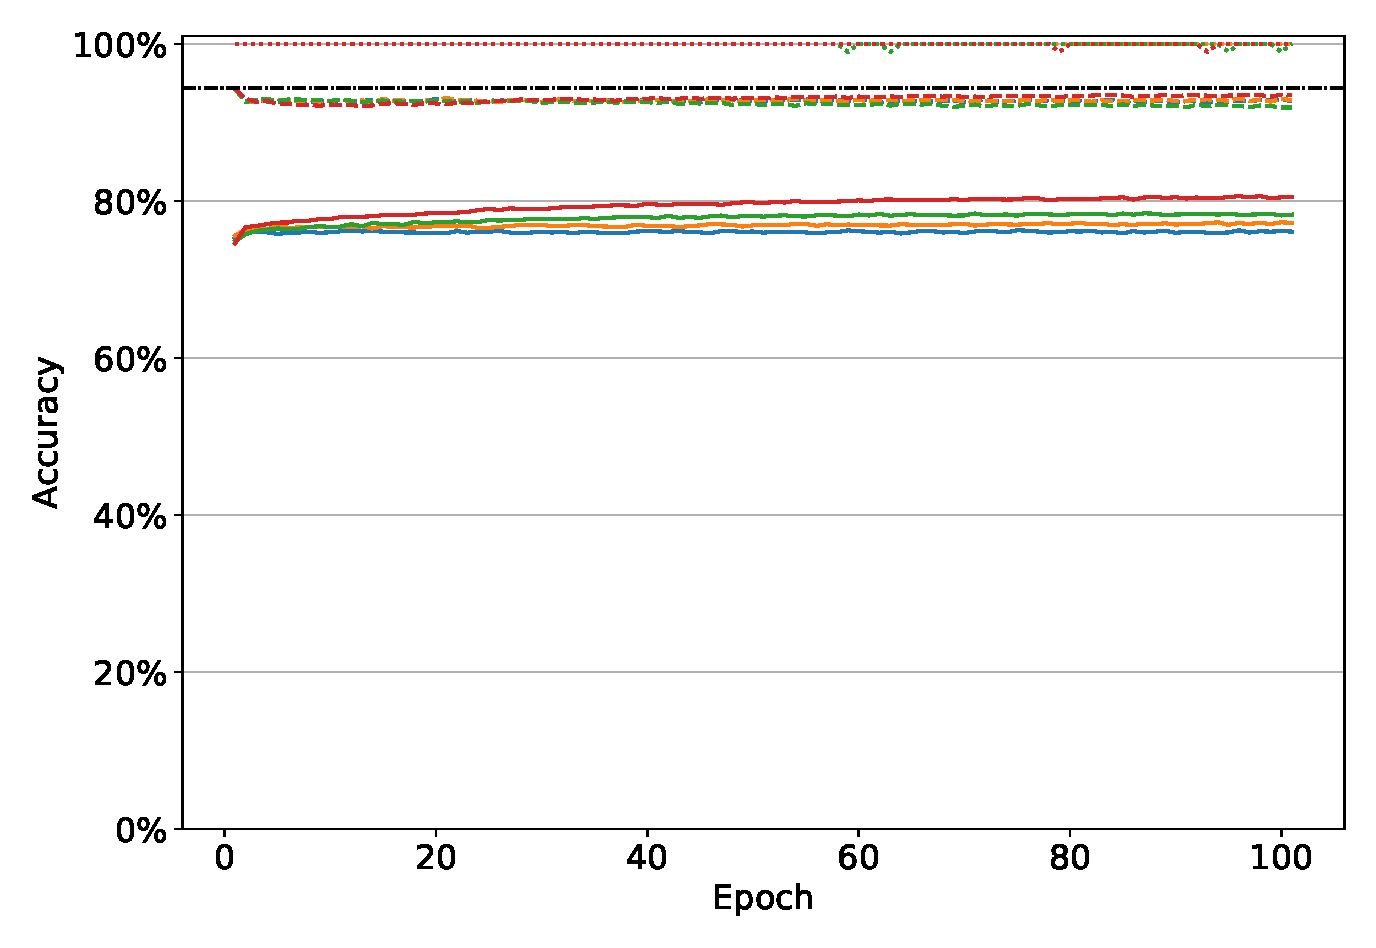
\includegraphics[width=\textwidth]{images/finetuning/finetuning_protecting_content_smalllr_thesis_resnet50.eps}
         \caption{ResNet-50}
         \label{fig:finetuning_resnet50_smalllr}
     \end{subfigure}
     \hfill
     \begin{subfigure}[b]{0.49\textwidth}
         \centering
         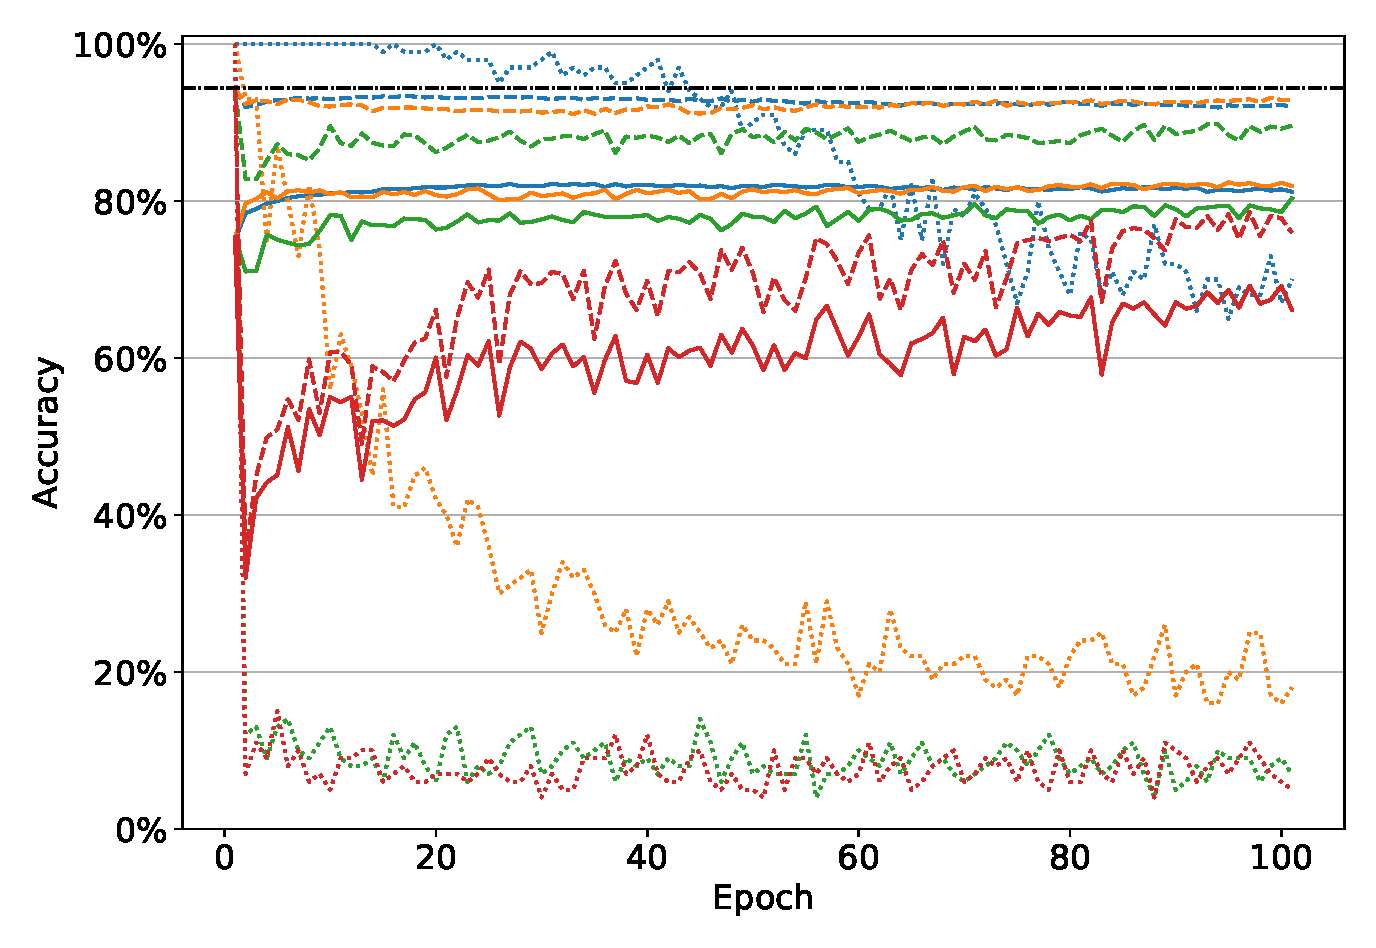
\includegraphics[width=\textwidth]{images/finetuning/finetuning_protecting_content_largelr_thesis_resnet50.eps}
         \caption{ResNet-50}
         \label{fig:finetuning_resnet50_largelr}
     \end{subfigure}
     \hfill
     
     \begin{subfigure}[b]{\textwidth}
         \centering
         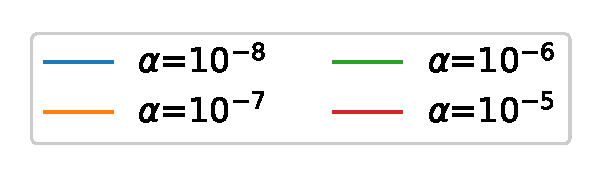
\includegraphics[height=1cm]{images/finetuning/legend_content_finetuning_smalllr_colors.eps}
         \quad
         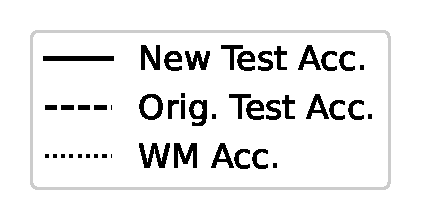
\includegraphics[height=1.3cm]{images/finetuning/legend_content_finetuning_linetypes.eps}
         \quad
         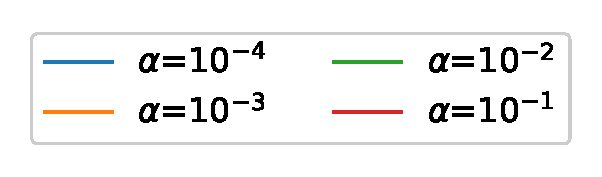
\includegraphics[height=1cm]{images/finetuning/legend_content_finetuning_largelr_colors.eps}
     \end{subfigure}
     
     \caption{Fine-tuning on \textbf{CIFAR-10} models, watermarked with \textit{ProtectingIP-pattern}. The plots on the left side correspond to fine-tuning with smaller learning rates and the ones on the right side to fine-tuning with larger learning rates. The black dash-dotted line corresponds to the benchmark test accuracy of the non-watermarked model.}
     \label{fig:finetuning_cifar10models}
\end{figure}


\begin{figure}
\centering
\begin{subfigure}[b]{0.49\textwidth}
    \centering
    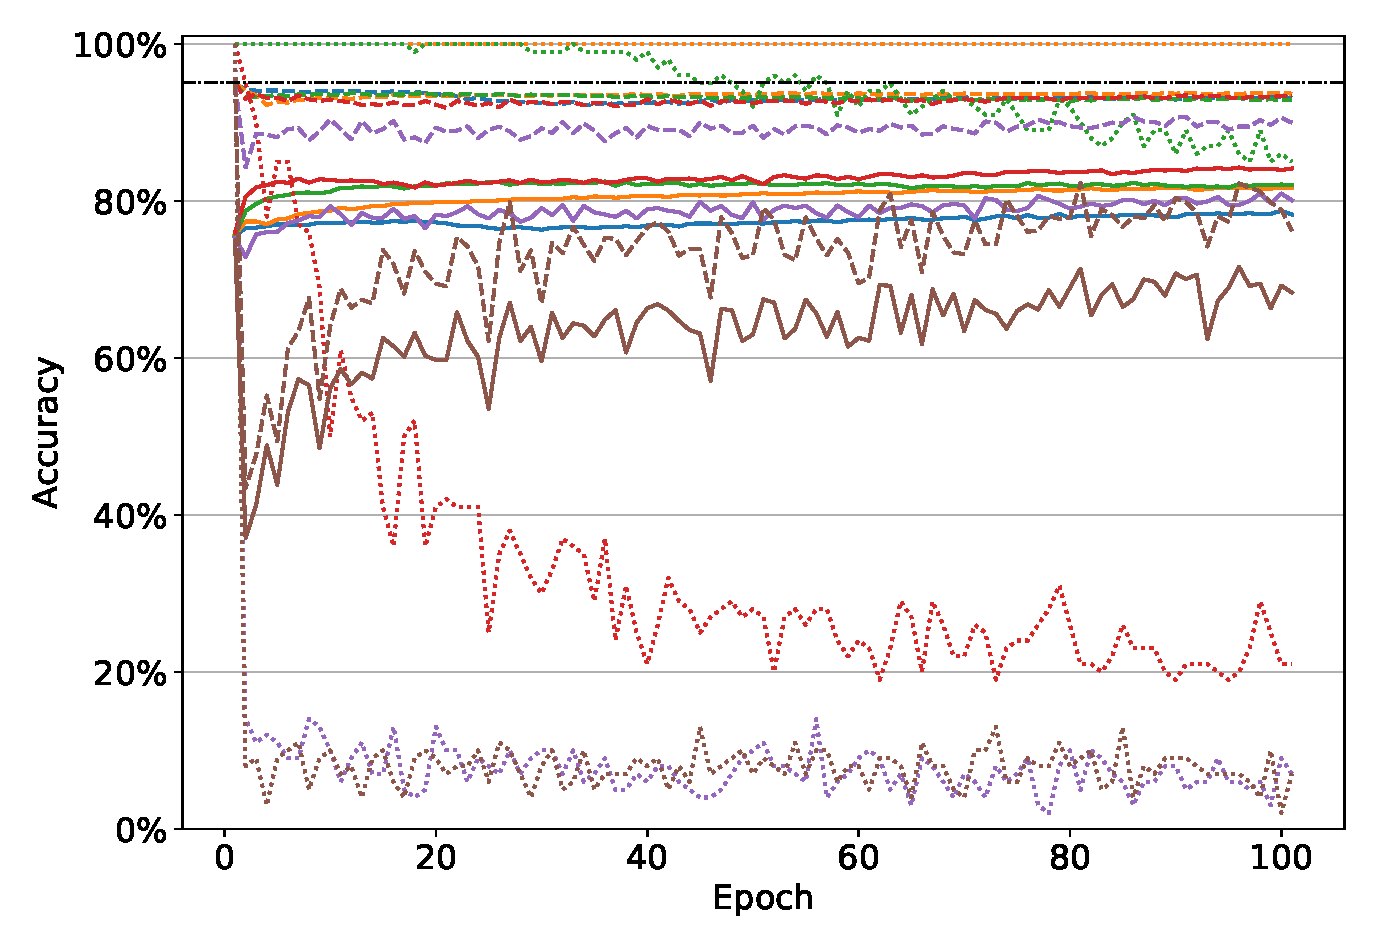
\includegraphics[width=\linewidth]{images/finetuning/finetuning_protecting_content_imagenet_0.eps}
    \caption{Fine-Tuning on CINIC-10}
\end{subfigure}
\begin{subfigure}[b]{0.49\textwidth}
    \centering
    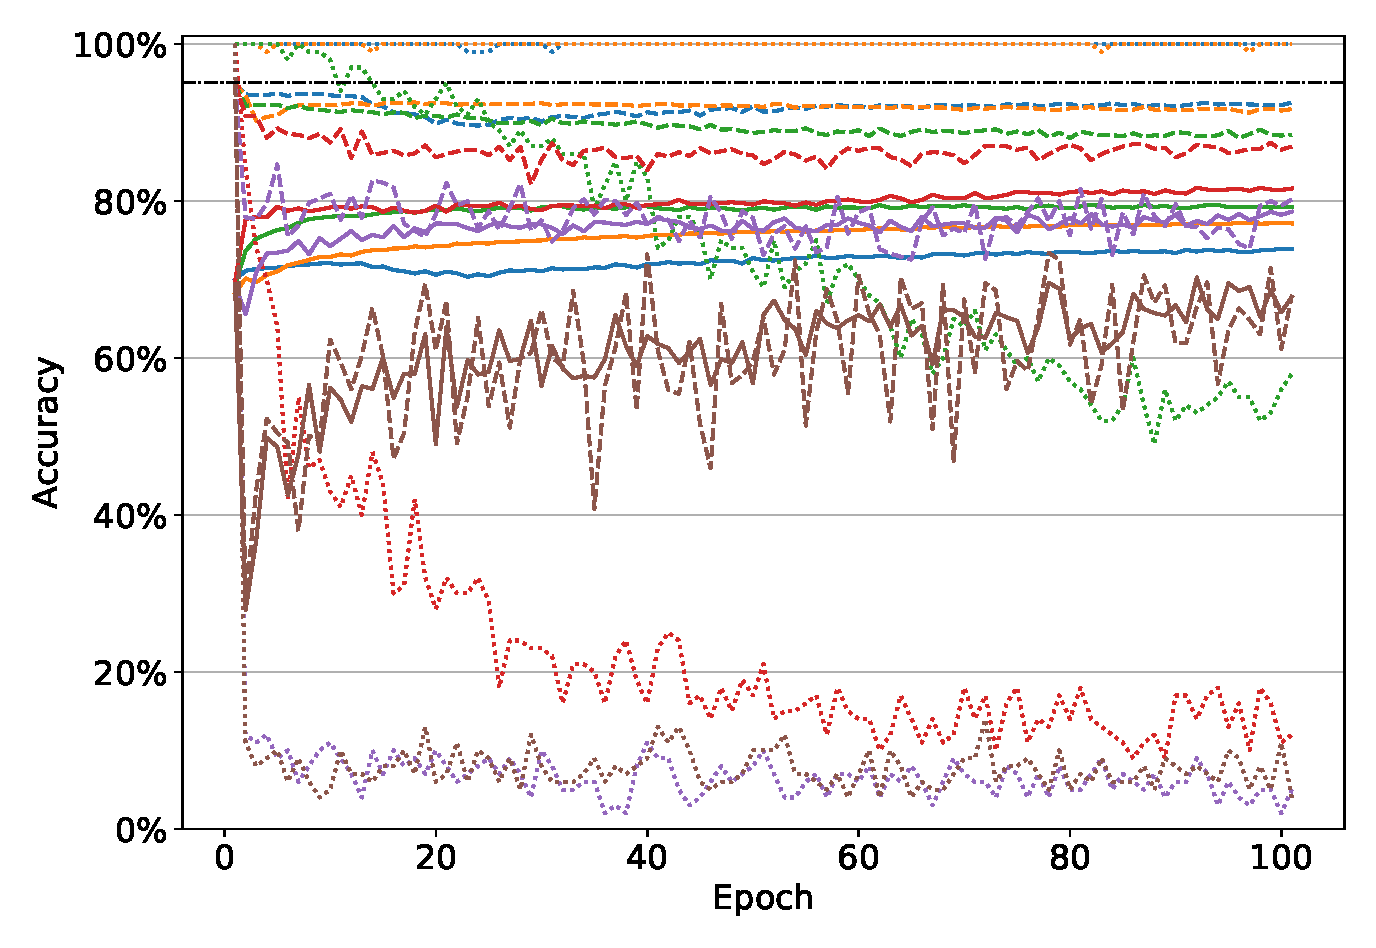
\includegraphics[width=\linewidth]{images/finetuning/finetuning_protecting_content_imagenet_1.eps}
    \caption{Fine-Tuning on ImageNet part of CINIC-10}
\end{subfigure}

\begin{subfigure}[b]{\linewidth}
    \centering
    \includegraphics[height=1.1cm]{images/finetuning/legend_content_finetuning_imagenet_colors.eps}
    \quad
    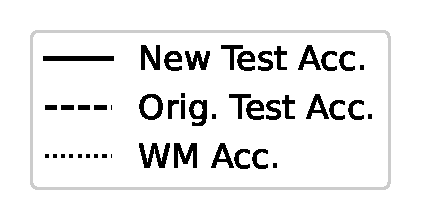
\includegraphics[height=1.1cm]{images/finetuning/legend_content_finetuning_imagenet_linetypes.eps}
\end{subfigure}

\caption{Fine-Tuning on both, CINIC-10 and only on the ImageNet part of CINIC-10. Original line plots to \cref{fig:fine-tuning-both-cinic10-imagenet}.}
\label{fig:fine-tuning-both-cinic10-imagenet-original}

\end{figure}
%\clearpage
%\section{Results for plots}
%\begin{table}
\centering
\small
\caption{Additional experiments for \textit{FrontierStitching}, varying $\epsilon$: fidelity}
\label{tab:results_frontier_fidelity}
\begin{tabular}{|l|l|l||l|l|l|}
\hline
\multicolumn{3}{|c|}{\textbf{CIFAR-10}}     & \multicolumn{3}{c|}{\textbf{MNIST}}         \\ \hline
Arch      & $\epsilon$    & Rel. valid. loss diff. & Arch      & $\epsilon$    & Rel. valid. loss diff. \\ \hline
DenseNet  & 0.0001 & 0.2342                 & SimpleNet & 0.0001 & 0.1551                 \\ \hline
          & 0.001  & 0.3298                 &           & 0.001  & 0.0785                 \\ \hline
          & 0.01   & 0.289                  &           & 0.01   & 0.1363                 \\ \hline
          & 0.1    & 0.3605                 &           & 0.1    & 0.1184                 \\ \hline
          & 0.25   & 0.3394                 &           & 0.25   & 0.144                  \\ \hline
          & 0.5    & 0.2996                 &           & 0.5    & 0.1635                 \\ \hline
          & 1      & 0.3394                 &           & 1      & 0.0776                 \\ \hline
ResNet-18 & 0.0001 & 0.1966                 & LeNet-1   & 0.0001 & 1.0639                 \\ \hline
          & 0.001  & 0.1521                 &           & 0.001  & 1.1265                 \\ \hline
          & 0.01   & 0.1837                 &           & 0.01   & 0.5238                 \\ \hline
          & 0.1    & 0.1739                 &           & 0.1    & 0.4911                 \\ \hline
          & 0.25   & 0.1441                 &           & 0.25   & 0.4376                 \\ \hline
          & 0.5    & 0.095                  &           & 0.5    & 0.0765                 \\ \hline
          & 1      & 0.1378                 &           & 1      & 0.013                  \\ \hline
ResNet-34 & 0.0001 & 0.0689                 & LeNet-3   & 0.0001 & 1.3487                 \\ \hline
          & 0.001  & 0.1154                 &           & 0.001  & 1.2401                 \\ \hline
          & 0.01   & 0.0844                 &           & 0.01   & 1.3268                 \\ \hline
          & 0.1    & 0.0311                 &           & 0.1    & 0.6569                 \\ \hline
          & 0.25   & 0.0815                 &           & 0.25   & 0.7123                 \\ \hline
          & 0.5    & 0.1141                 &           & 0.5    & 0.285                  \\ \hline
          & 1      & 0.0906                 &           & 1      & 0.127                  \\ \hline
ResNet-50 & 0.0001 & 0.0463                 & LeNet-5   & 0.0001 & 1.0773                 \\ \hline
          & 0.001  & 0.1331                 &           & 0.001  & 1.1608                 \\ \hline
          & 0.01   & 0.1566                 &           & 0.01   & 1.2101                 \\ \hline
          & 0.1    & 0.0892                 &           & 0.1    & 0.7567                 \\ \hline
          & 0.25   & 0.0971                 &           & 0.25   & 0.5123                 \\ \hline
          & 0.5    & 0.1807                 &           & 0.5    & 0.3898                 \\ \hline
          & 1      & 0.2041                 &           & 1      & 0.1825                 \\ \hline
\end{tabular}
\end{table}
%\begin{table}
\centering

\caption{Additional experiments for \textit{FrontierStitching}, varying $\epsilon$: pruning}
\label{tab:results_frontier_pruning}

\setlength\tabcolsep{2pt}
\renewcommand{\arraystretch}{1.2}

\resizebox{\textwidth}{!}{
\begin{tabular}{|l|l|c|c|c|c|c|c|c|c|c|c|c|c|c|c|c|c|c|c|}
\hline
          &  & \multicolumn{2}{c|}{0.1} & \multicolumn{2}{c|}{0.2} & \multicolumn{2}{c|}{0.3} & \multicolumn{2}{c|}{0.4} & \multicolumn{2}{c|}{0.5} & \multicolumn{2}{c|}{0.6} & \multicolumn{2}{c|}{0.7} & \multicolumn{2}{c|}{0.8} & \multicolumn{2}{c|}{0.9} \\ \hline
Arch      & $\epsilon$      & Test         & WM        & Test         & WM        & Test         & WM        & Test         & WM        & Test         & WM        & Test         & WM        & Test         & WM        & Test         & WM        & Test         & WM        \\ \hline
DenseNet  & 0.0001   & 93.01        & 100       & 93.01        & 100       & 93.01        & 100       & 93.01        & 100       & 93.01        & 100       & 93.01        & 100       & 93.01        & 100       & 93.01        & 100       & 92.45        & 100       \\ \hline
          & 0.001    & 92.47        & 100       & 92.47        & 100       & 92.47        & 100       & 92.47        & 100       & 92.47        & 100       & 92.47        & 100       & 92.47        & 100       & 92.47        & 100       & 92.38        & 100       \\ \hline
          & 0.01     & 92.41        & 100       & 92.41        & 100       & 92.41        & 100       & 92.41        & 100       & 92.41        & 100       & 92.41        & 100       & 92.41        & 100       & 92.41        & 100       & 92.02        & 100       \\ \hline
          & 0.1      & 92.19        & 100       & 92.19        & 100       & 92.19        & 100       & 92.19        & 100       & 92.19        & 100       & 92.19        & 100       & 92.19        & 100       & 92.19        & 100       & 91.67        & 100       \\ \hline
          & 0.25     & 92.41        & 100       & 92.41        & 100       & 92.41        & 100       & 92.41        & 100       & 92.41        & 100       & 92.41        & 100       & 92.41        & 100       & 92.41        & 100       & 91.89        & 100       \\ \hline
          & 0.5      & 92.74        & 100       & 92.74        & 100       & 92.74        & 100       & 92.74        & 100       & 92.74        & 100       & 92.74        & 100       & 92.74        & 100       & 92.74        & 100       & 91.94        & 100       \\ \hline
          & 1        & 91.09        & 100       & 91.09        & 100       & 91.09        & 100       & 91.09        & 100       & 91.09        & 100       & 91.09        & 100       & 91.09        & 100       & 91.09        & 100       & 90.42        & 99        \\ \hline
ResNet-18 & 0.0001   & 94.13        & 100       & 94.13        & 100       & 94.13        & 100       & 94.13        & 100       & 94.14        & 100       & 94.2         & 100       & 93.97        & 100       & 93.25        & 100       & 51.3         & 32        \\ \hline
          & 0.001    & 94.7         & 100       & 94.7         & 100       & 94.7         & 100       & 94.7         & 100       & 94.7         & 100       & 94.75        & 100       & 94.68        & 100       & 94.22        & 100       & 83.61        & 88        \\ \hline
          & 0.01     & 94.54        & 100       & 94.54        & 100       & 94.54        & 100       & 94.54        & 100       & 94.54        & 100       & 94.57        & 100       & 94.61        & 100       & 94.25        & 100       & 79.63        & 74        \\ \hline
          & 0.1      & 94.81        & 100       & 94.81        & 100       & 94.81        & 100       & 94.81        & 100       & 94.81        & 100       & 94.77        & 100       & 94.75        & 100       & 94.13        & 100       & 68.29        & 76        \\ \hline
          & 0.25     & 94.54        & 100       & 94.54        & 100       & 94.54        & 100       & 94.54        & 100       & 94.54        & 100       & 94.53        & 100       & 94.55        & 100       & 94.2         & 100       & 62.21        & 73        \\ \hline
          & 0.5      & 94.7         & 100       & 94.7         & 100       & 94.7         & 100       & 94.7         & 100       & 94.7         & 100       & 94.73        & 100       & 94.71        & 100       & 94.44        & 100       & 83.08        & 86        \\ \hline
          & 1        & 94.24        & 100       & 94.24        & 100       & 94.24        & 100       & 94.24        & 100       & 94.23        & 100       & 94.2         & 100       & 94.15        & 100       & 93.59        & 100       & 67.88        & 90        \\ \hline
ResNet-34 & 0.0001   & 94.7         & 100       & 94.7         & 100       & 94.7         & 100       & 94.7         & 100       & 94.7         & 100       & 94.7         & 100       & 94.71        & 100       & 94.68        & 100       & 93.95        & 100       \\ \hline
          & 0.001    & 94.52        & 100       & 94.52        & 100       & 94.52        & 100       & 94.52        & 100       & 94.52        & 100       & 94.52        & 100       & 94.52        & 100       & 94.45        & 100       & 93.86        & 100       \\ \hline
          & 0.01     & 95.11        & 100       & 95.11        & 100       & 95.11        & 100       & 95.11        & 100       & 95.11        & 100       & 95.11        & 100       & 95.12        & 100       & 95.12        & 100       & 94.37        & 100       \\ \hline
          & 0.1      & 95.19        & 100       & 95.19        & 100       & 95.19        & 100       & 95.19        & 100       & 95.19        & 100       & 95.2         & 100       & 95.21        & 100       & 95.21        & 100       & 93.94        & 100       \\ \hline
          & 0.25     & 95.27        & 100       & 95.27        & 100       & 95.27        & 100       & 95.27        & 100       & 95.27        & 100       & 95.27        & 100       & 95.25        & 100       & 95.19        & 100       & 94.92        & 100       \\ \hline
          & 0.5      & 94.7         & 100       & 94.7         & 100       & 94.7         & 100       & 94.7         & 100       & 94.7         & 100       & 94.7         & 100       & 94.71        & 100       & 94.73        & 100       & 93.53        & 100       \\ \hline
          & 1        & 94.14        & 100       & 94.14        & 100       & 94.14        & 100       & 94.14        & 100       & 94.14        & 100       & 94.15        & 100       & 94.18        & 100       & 94.21        & 100       & 93.55        & 100       \\ \hline
ResNet-50 & 0.0001   & 94.49        & 100       & 94.49        & 100       & 94.49        & 100       & 94.49        & 100       & 94.49        & 100       & 94.49        & 100       & 94.49        & 100       & 94.48        & 100       & 93.21        & 96        \\ \hline
          & 0.001    & 94.41        & 100       & 94.41        & 100       & 94.41        & 100       & 94.41        & 100       & 94.41        & 100       & 94.41        & 100       & 94.4         & 100       & 94.41        & 100       & 93.9         & 100       \\ \hline
          & 0.01     & 93.98        & 100       & 93.98        & 100       & 93.98        & 100       & 93.98        & 100       & 93.98        & 100       & 93.98        & 100       & 93.97        & 100       & 93.97        & 100       & 93.55        & 100       \\ \hline
          & 0.1      & 93.54        & 100       & 93.54        & 100       & 93.54        & 100       & 93.54        & 100       & 93.54        & 100       & 93.54        & 100       & 93.54        & 100       & 93.54        & 100       & 93.19        & 100       \\ \hline
          & 0.25     & 64.02        & 99        & 64.02        & 99        & 64.02        & 99        & 64.02        & 99        & 64.02        & 99        & 64.03        & 99        & 64.05        & 100       & 64.2         & 100       & 63.46        & 99        \\ \hline
          & 0.5      & 93.44        & 100       & 93.44        & 100       & 93.44        & 100       & 93.44        & 100       & 93.44        & 100       & 93.44        & 100       & 93.44        & 100       & 93.38        & 100       & 93.22        & 100       \\ \hline
          & 1        & 94           & 100       & 94           & 100       & 94           & 100       & 94           & 100       & 94           & 100       & 94           & 100       & 94.01        & 100       & 94.04        & 100       & 93.69        & 100       \\ \hline
SimpleNet & 0.0001   & 99.54        & 100       & 99.54        & 100       & 99.54        & 100       & 99.55        & 100       & 99.55        & 100       & 99.55        & 100       & 99.56        & 100       & 99.49        & 100       & 36.47        & 65        \\ \hline
          & 0.001    & 99.58        & 100       & 99.58        & 100       & 99.58        & 100       & 99.58        & 100       & 99.58        & 100       & 99.57        & 100       & 99.55        & 100       & 99.5         & 100       & 41.51        & 73        \\ \hline
          & 0.01     & 99.55        & 100       & 99.55        & 100       & 99.55        & 100       & 99.53        & 100       & 99.55        & 100       & 99.53        & 100       & 99.5         & 100       & 99.24        & 100       & 40.76        & 75        \\ \hline
          & 0.1      & 99.57        & 100       & 99.57        & 100       & 99.57        & 100       & 99.58        & 100       & 99.58        & 100       & 99.57        & 100       & 99.55        & 100       & 99.33        & 100       & 56.08        & 63        \\ \hline
          & 0.25     & 99.65        & 100       & 99.65        & 100       & 99.65        & 100       & 99.65        & 100       & 99.64        & 100       & 99.63        & 100       & 99.61        & 100       & 99.45        & 100       & 57.57        & 58        \\ \hline
          & 0.5      & 99.64        & 100       & 99.64        & 100       & 99.64        & 100       & 99.64        & 100       & 99.66        & 100       & 99.65        & 100       & 99.6         & 100       & 99.19        & 100       & 46.55        & 49        \\ \hline
          & 1        & 99.54        & 100       & 99.54        & 100       & 99.54        & 100       & 99.54        & 100       & 99.54        & 100       & 99.55        & 100       & 99.54        & 100       & 98.94        & 100       & 55.85        & 61        \\ \hline
LeNet-1   & 0.0001   & 97.67        & 100       & 97.45        & 100       & 96.99        & 98        & 95.58        & 84        & 87.1         & 61        & 65           & 43        & 67.3         & 32        & 51.34        & 31        & 29.25        & 20        \\ \hline
          & 0.001    & 97.97        & 100       & 97.96        & 99        & 97.24        & 93        & 96.34        & 83        & 93.38        & 64        & 89.48        & 40        & 83.47        & 35        & 44.82        & 37        & 27.59        & 19        \\ \hline
          & 0.01     & 98.29        & 100       & 98.27        & 100       & 98.14        & 100       & 97.86        & 100       & 97.3         & 88        & 93.25        & 66        & 91.67        & 64        & 80.25        & 37        & 24.71        & 18        \\ \hline
          & 0.1      & 98.32        & 100       & 98.25        & 100       & 98.22        & 100       & 97.86        & 98        & 97.46        & 90        & 94.95        & 76        & 82.93        & 46        & 67.46        & 41        & 31.22        & 21        \\ \hline
          & 0.25     & 98.52        & 100       & 98.53        & 100       & 98.51        & 100       & 98.3         & 100       & 97.84        & 96        & 96.36        & 81        & 93.81        & 75        & 81.9         & 42        & 26.41        & 13        \\ \hline
          & 0.5      & 98.7         & 100       & 98.69        & 100       & 98.6         & 100       & 98.39        & 100       & 96.95        & 98        & 96.01        & 91        & 84.82        & 64        & 80.16        & 43        & 23.43        & 26        \\ \hline
          & 1        & 98.71        & 100       & 98.71        & 100       & 98.68        & 100       & 98.27        & 100       & 97.39        & 90        & 96.77        & 88        & 95.48        & 60        & 87.75        & 33        & 51           & 32        \\ \hline
LeNet-3   & 0.0001   & 98.38        & 100       & 98.38        & 100       & 98.38        & 100       & 98.38        & 100       & 98.38        & 100       & 98.37        & 100       & 98.36        & 100       & 98.32        & 100       & 97.44        & 62        \\ \hline
          & 0.001    & 98.63        & 100       & 98.63        & 100       & 98.63        & 100       & 98.63        & 100       & 98.63        & 100       & 98.63        & 100       & 98.62        & 100       & 98.55        & 100       & 97.03        & 73        \\ \hline
          & 0.01     & 98.64        & 100       & 98.64        & 100       & 98.64        & 100       & 98.64        & 100       & 98.64        & 100       & 98.65        & 100       & 98.63        & 100       & 98.65        & 100       & 97.24        & 59        \\ \hline
          & 0.1      & 98.99        & 100       & 98.99        & 100       & 98.99        & 100       & 98.99        & 100       & 98.99        & 100       & 98.99        & 100       & 99.02        & 100       & 98.92        & 100       & 98.29        & 89        \\ \hline
          & 0.25     & 98.84        & 100       & 98.84        & 100       & 98.84        & 100       & 98.84        & 100       & 98.84        & 100       & 98.84        & 100       & 98.86        & 100       & 98.82        & 100       & 98.57        & 90        \\ \hline
          & 0.5      & 98.95        & 100       & 98.95        & 100       & 98.95        & 100       & 98.95        & 100       & 98.95        & 100       & 98.95        & 100       & 98.97        & 100       & 98.96        & 100       & 98.62        & 74        \\ \hline
          & 1        & 99.1         & 100       & 99.1         & 100       & 99.1         & 100       & 99.1         & 100       & 99.1         & 100       & 99.1         & 100       & 99.12        & 100       & 99.05        & 100       & 98.54        & 66        \\ \hline
LeNet-5   & 0.0001   & 98.56        & 100       & 98.56        & 100       & 98.56        & 100       & 98.56        & 100       & 98.57        & 100       & 98.59        & 100       & 98.55        & 100       & 98.33        & 94        & 97.1         & 49        \\ \hline
          & 0.001    & 98.58        & 100       & 98.58        & 100       & 98.58        & 100       & 98.58        & 100       & 98.58        & 100       & 98.51        & 100       & 98.62        & 100       & 98.61        & 93        & 96.84        & 43        \\ \hline
          & 0.01     & 98.86        & 100       & 98.86        & 100       & 98.86        & 100       & 98.86        & 100       & 98.85        & 100       & 98.83        & 100       & 98.9         & 100       & 98.73        & 86        & 97.53        & 49        \\ \hline
          & 0.1      & 98.89        & 100       & 98.89        & 100       & 98.89        & 100       & 98.89        & 100       & 98.89        & 100       & 98.9         & 100       & 98.92        & 100       & 98.83        & 99        & 97.71        & 58        \\ \hline
          & 0.25     & 98.83        & 68        & 98.83        & 68        & 98.83        & 68        & 98.83        & 68        & 98.83        & 68        & 98.86        & 67        & 98.83        & 67        & 98.7         & 63        & 98.25        & 52        \\ \hline
          & 0.5      & 99           & 100       & 99           & 100       & 99           & 100       & 99           & 100       & 99           & 100       & 99           & 100       & 99.04        & 100       & 98.94        & 100       & 98.02        & 70        \\ \hline
          & 1        & 99.06        & 100       & 99.06        & 100       & 99.06        & 100       & 99.06        & 100       & 99.06        & 100       & 99.05        & 100       & 99.09        & 100       & 99.08        & 99        & 98.49        & 59        \\ \hline
\end{tabular}
}
\end{table}